\documentclass{article}

% general packages
\usepackage{url}
\usepackage{graphicx}
\usepackage{mathtools}  % math tools
\usepackage{caption}    % support subfigure
\usepackage{subcaption} % support subfigure
\usepackage{placeins}   % support FloatBarrier
\usepackage{listings}   % support codes
\usepackage{color}      % support color
\usepackage{amsmath} 	% support multiple lines
\usepackage{amsfonts,amssymb} % support holo characters
\usepackage[10pt]{extsizes}
%\documentstyle[nips14submit_09,times,art10]{article} % For LaTeX 2.09

%-----------------------------------------------
% special packages

\usepackage[numbers,sort&compress]{natbib}		% 文献引用连号时[1,2,3]变成[1-3]
\usepackage{fancyhdr} 					% 加载fancyhdr宏包
\usepackage[hidelinks]{hyperref}        % 支持超链接(隐藏超链接效果)
\usepackage{multirow} 					% 多行表格
\usepackage{float} 						% 图片禁止浮动
\usepackage{geometry}
%\usepackage{CJKutf8} 					% 支持中文——方案1(不支持中文页眉而放弃)
\usepackage[UTF8]{ctex}  				% 支持中文——方案2
\usepackage{makecell} 					% 单单元格调整
\usepackage{longtable} 					% 表格——跨页面
\usepackage{tabularx} 					% 表格——自动调整列宽
\usepackage{array} 						% 表格——用于 \newcolumntype
\usepackage{makecell} 					% 表格——独立表格
\usepackage[table]{xcolor}  			% 加载xcolor宏包,启用表格颜色功能
\usepackage{pifont} 					% 圆圈1-20: \ding{172} -\ding{181} 
\usepackage{algorithm, algpseudocode} 	% 伪代码
\usepackage{underscore} 				% 下划线
\usepackage{ulem} 					% 文字划线等
\usepackage{svg} 								% 支持SVG图片
\usepackage{bm}									%
\usepackage{enumitem}							% item支持更多格式
\usepackage[numbers,sort&compress]{natbib}		% 文献引用连号时[1,2,3]变成[1-3]
\usepackage{breqn}								% 公式过长自动换行

%-----------------------------------------------
% page settings
\geometry{a4paper,left=2cm,right=2cm,top=2cm,bottom=2cm}
\renewcommand{\baselinestretch}{1.2}
\setlength{\parindent}{0pt} % 设置段落缩进为 0
% 定义页眉风格
\pagestyle{fancy} 
\fancyhead[L]{} % 设置左页眉
\fancyhead[C]{Qu's Joint Channle Estimation \& Symbol Detection} % 设置中页眉
\fancyhead[R]{} % 设置右页眉
\renewcommand{\headrulewidth}{0.4pt} % 设置页眉线宽度(可选)

%-----------------------------------------------
% set math notations
\DeclarePairedDelimiter{\norm}{\lVert}{\rVert}
% paths 
\graphicspath{{../../img/}}
% define color
\definecolor{darkred}{rgb}{0.6,0.0,0.0}
\definecolor{darkgreen}{rgb}{0,0.50,0}
\definecolor{lightblue}{rgb}{0.0,0.42,0.91}
\definecolor{orange}{rgb}{0.99,0.48,0.13}
\definecolor{grass}{rgb}{0.18,0.80,0.18}
\definecolor{pink}{rgb}{0.97,0.15,0.45}
\definecolor{lightgreen}{RGB}{220, 255, 220}  % 浅绿色
\definecolor{lightred}{RGB}{255, 220, 220}    % 浅红色

%-----------------------------------------------
% 其他自定义设置
% 覆盖 breqn 的编号设置
\renewcommand{\theequation}{\arabic{equation}}

% 定义不同宽度的列类型
%\newcolumntype{TBX}{>{\hsize=1\hsize\centering\arraybackslash}X}
%\newcolumntype{MyCol}{>{\hsize=1.5\hsize\centering\arraybackslash}X}
%\newcolumntype{TBL}{>{\hsize=2\hsize\arraybackslash}X}
% 允许跨页
\allowdisplaybreaks[4]
% 设置标题编号深度,使其出现在目录中(如果需要)
\setcounter{secnumdepth}{4}
\setcounter{tocdepth}{4} % 如果你也希望它出现在目录中
% 伪代码
% 伪代码——跨行
\makeatletter
\newenvironment{breakablealgorithm}
  {% \begin{breakablealgorithm}
   \begin{center}
     \refstepcounter{algorithm}% New algorithm
     \hrule height.8pt depth0pt \kern2pt% \@fs@pre for \@fs@ruled
     \renewcommand{\caption}[2][\relax]{% Make a new \caption
       {\raggedright\textbf{\ALG@name~\thealgorithm} ##2\par}%
       \ifx\relax##1\relax % #1 is \relax
         \addcontentsline{loa}{algorithm}{\protect\numberline{\thealgorithm}##2}%
       \else % #1 is not \relax
         \addcontentsline{loa}{algorithm}{\protect\numberline{\thealgorithm}##1}%
       \fi
       \kern2pt\hrule\kern2pt
     }
  }{% \end{breakablealgorithm}
     \kern2pt\hrule\relax% \@fs@post for \@fs@ruled
   \end{center}
  }
\makeatother
% 伪代码——注释
\renewcommand{\algorithmiccomment}[1]{\hfill // #1}


%% 自定义字符
\newcommand{\T}{^{\mathrm{T}}} % 转置
\newcommand{\HT}{^{\mathrm{H}}} % 共轭转置
\newcommand{\diag}{{\sf diag}} % 生成对角矩阵
\newcommand{\off}{{\sf off}} % 对角元素置0
\newcommand{\vect}{{\sf vec}} % 向量化
\input{./authors}

% version
\newcommand{\version}{v1.0.2}
% paths 
\graphicspath{{../img/}}

%-----------------------------------------------
% title
% 
\title{
	\Huge \textbf{Variational Bayes} \\[1em]
}
\author{\qxw}
\date{\today}

%-----------------------------------------------
% document
%
\begin{document}
% \begin{CJK}{UTF8}{gbsn} % 不支持中文页眉而放弃

\maketitle

\newpage
\tableofcontents
\newpage

\section{Common Distributions}
\subsection{Gamma Distribution}
Supposing we have a gamma distribution $p(x; a, b)$. $a$表示事件次数,$b$表示每次发生的概率。The probability density function (PDF) of gamma distribution is
\[
p(x) = \frac{x^{(a-1)}b^ae^{-bx}}{\Gamma(a)}
\] 
\[
\text{ln} p(x) \propto (a-1)ln(x) - bx
\]
The mean is
\[
\mu_x = \frac{a}{b}
\]
The variance is
\begin{equation}
\sigma^2_x = \frac{a}{b^2}
\end{equation}
\subsection{Complex Gaussian Distribution}
\begin{itemize}
\item For a complex Gaussian distributed variable $x$, its PDF is
\[
p(x) = \frac{1}{\pi\sigma^2}e^{-\frac{|x-\mu|^2}{\sigma^2}}
\]
\begin{align}
lnp(x) \propto  -ln(\sigma^2) - \sigma^{-2}|x-\mu|^2
\end{align}

\item For a complex Gaussian distributed variable vector $x = [x_0, \cdots, x_{N-1}]$, its PDF is
\[
p(x) = \frac{1}{\pi^N det(\Sigma)}e^{-(x-\mu)^H\Sigma^{-1}(x-\mu)}
\]
\begin{align}
lnp(x) \propto  -lndet(\Sigma) - (x-\mu)^H\Sigma^{-1}(x-\mu)
\end{align}
where $\Sigma$ is the covariance matrix.
\end{itemize}




\section{Variational Bayes}
For a telecommunication system, we have
\begin{equation}
y = Hx + z,
\end{equation}
where $y$ is the received signal, $x$ is the transmitted signal and $z\in \mathcal{CN}(0, \sigma^2)$. Please note that, 
\begin{equation}
x = x_p + x_d,
\end{equation}
where $x_p$ is the pilot and $x_d$ is data.
\subsection{Bayes Interference}
In the Rx, given the prior $p(y)$, we compute posterior distribution $p(y|x)$,
\begin{equation}
p(x|y) = \frac{p(x,y)}{p(y)} = \frac{\overbrace{p(y|x)}^{likelihood}\overbrace{p(x)}^{prior}}{\underbrace{p(y)}_{evidence}} = \frac{p(y|x)p(x)}{\int_y p(x,y)dy}
\end{equation}
Usually, we assume the evidence is 100\%, i.e., $p(y)=1$. Hence,
\begin{equation}
p(x|y) \propto \overbrace{p(y|x)}^{likelihood}\overbrace{p(x)}^{prior}
\end{equation}
Here, we need to choose \colorbox{yellow}{the likelihood and the prior}.
\subsection{Variational Interference}
However, the posterior may have no closed form, i.e., computing $p(x|y)$ is not feasible. Instead, we use a distribution $Q$ over the symbols $x$ to approximate $p(x|y)$, i.e.,
\begin{equation}
\begin{split}
q^*(x) &= \mathop{\arg\min}\limits_{q(x)\in Q} KL(q(x) || p(x|y)) \\
&= \mathop{\arg\min}\limits_{q(x)\in Q} \int_{x}q(x)\text{ln} \frac{q(x)}{p(x|y)}dx \\
&= \mathop{\arg\min}\limits_{q(x)\in Q} -\int_{x}q(x)\text{ln} \frac{p(x|y)}{q(x)}dx
\end{split}
\end{equation}
Here, $q^*(x)$ is the optimal $q(x)$ but \colorbox{yellow}{$p(x|y)$ is unknown}. Herefore,
\begin{align}
KL(q(x) || p(x|y)) &= -\int_{x}q(x)\text{ln} \frac{p(x|y)}{q(x)}dx \\
&= \int_{x}q(x)\text{ln} q(x)dx - \int_{x}q(x)\text{ln}  p(x|y)dx \\ 
&= \int_{x}q(x)\text{ln} q(x)dx - \int_{x}q(x)\text{ln}  \frac{p(x,y)}{p(y)}dx \\ 
&= \int_{x}q(x)\text{ln} q(x)dx - \int_{x}q(x)\text{ln}p(x,y)dx + \int_{x}q(x)\text{ln}p(y)dx \\ 
&= \int_{x}q(x)\text{ln} q(x)dx - \int_{x}q(x)\text{ln}p(x,y)dx + \text{ln}p(y)\int_{x}q(x)dx \\ 
&= \underbrace{\mathbb{E}_q [\text{ln} q(x)] - \mathbb{E}_q[\text{ln}p(x,y)]}_{-ELBO} + \text{ln}p(y) \\
&= -ELBO(q) + \text{ln}p(y)
\label{eq:vb-vi-kl}
\end{align}
\subsubsection{ELBO}
Here, ELBO is Evidence Lower Bound, i.e.,
\begin{align}
ELBO(q) &= \mathbb{E}_q[\text{ln}p(x,y)] - \mathbb{E}_q [\text{ln} q(x)] \label{eq:vb-vi-elbo}\\ 
&= \int_x q(x)\text{ln}\frac{\overbrace{p(x,y)}^{known}}{q(x)}dx \\
&= \int_x q(x)\text{ln}\frac{p(y|x)p(x)}{q(x)}dx
\end{align}
\eqref{eq:vb-vi-kl} can be rewritten as,
\begin{equation}
\begin{split}
\underbrace{\text{ln}p(y)}_{\text{CONST}} &= ELBO(q) + \underbrace{KL(q(x) || p(x|y))}_{\geq 0} \\
&\geq ELBO(q)
\end{split}
\end{equation}
The minimizing KL can be taken as the maximizing ELBO, i.e.,
\begin{equation}
\begin{split}
q^*(x) &= \mathop{\arg\min}\limits_{q(x)\in Q} KL(q(x) || p(x|y)) \\
&= \mathop{\arg\max}\limits_{q(x)\in Q} ELBO(q) \\
\end{split}
\end{equation}
\subsection{Mean Field}
Now, we know the problem has been simplified as the maximizing ELBO. Here, we use the mean-field assumption, i.e.,
\begin{equation}
\begin{split}
q(x) &= \prod_{i=1}^m q_i(x_i) \\
\text{ln}q(x) &= \sum_{i=1}^m \text{ln}q_i(x_i) \\
\mathbb{E}_q [\text{ln} q(x)] &=   \sum_{i=1}^m\mathbb{E}_{q_i} [\text{ln} q_i(x_i)] 
\end{split}
\label{eq:vb-mf}
\end{equation}
\subsubsection{Coordinate Ascent Optimization}
In $q = [q_1, q_2, \cdots, q_j, \cdots, q_m]$, we fix others to update $q_j$, i.e.,
\begin{equation}
\begin{split}
q_j^*(x_j) &= \mathop{\arg\min}\limits_{q_j} ELBO(q_j) \\
&= \frac{\text{exp}\{\mathbb{E}_{q_{-j}}[\text{ln}p(x,y)]\}}{\int_{x_j}\text{exp}\{\mathbb{E}_{q_{-j}}[\text{ln}p(x,y)]\}dx_j}
\end{split}
\label{eq:vb-mf-cao}
\end{equation}
To prove \eqref{eq:vb-mf-cao}, we need to load \eqref{eq:vb-mf} into \eqref{eq:vb-vi-elbo},
\begin{align}
ELBO(q) &= \mathbb{E}_q[\text{ln}p(x,y)] - \mathbb{E}_q [\text{ln} q(x)] \\
&= \int_{x}q(x)\text{ln}p(x,y)dx - \left[\mathbb{E}_{q_j} [\text{ln} q_j(x_j)] + \sum_{i\neq j}\mathbb{E}_{q_i} [\text{ln} q_i(x_i)]\right]
\label{eq:vb-mf-cao-pf-1}
\end{align}
Here, $\sum_{i\neq j}\mathbb{E}_{q_i} [\text{ln} q_i(x_i)]$ can be seen as a constant because it is not related to $q_j$. Therefore, \eqref{eq:vb-mf-cao-pf-1} can be simplified as ($*_{-j}$ represents the other elements except $j$),
\begin{align}
ELBO(q) &= \int_{x}q(x)\text{ln}p(x,y)dx - \mathbb{E}_{q_j} [\text{ln} q_j(x_j)] + \text{const}\\
&=\int_{x}q(x)\text{ln}p(x,y)dx - \int_{x_j}q(x_j)\text{ln} q_j(x_j)dx_j + \text{const}\\
&=\int_{x_j}\int_{x_{-j}}q(x_j)q(x_{-j})\text{ln}p(x,y)dx_jdx_{-j} - \int_{x_j}q(x_j)\text{ln} q_j(x_j)dx_j + \text{const} \\
&= \int_{x_j}q(x_j)\left[\int_{x_{-j}}q(x_{-j})\text{ln}p(x,y)dx_{-j}\right]dx_j - \int_{x_j}q(x_j)\text{ln} q_j(x_j)dx_j + \text{const} \\
&= \int_{x_j}q(x_j)\mathbb{E}_{q_{-j}}[\text{ln}p(x,y)]dx_j - \int_{x_j}q(x_j)\text{ln} q_j(x_j)dx_j + \text{const}
\label{eq:vb-mf-cao-pf-2}
\end{align}
\colorbox{yellow}{Here, we define a new distribution}
\begin{equation}
\begin{split}
\text{ln}\tilde{p_j}(x_j,y) &= \mathbb{E}_{q_{-j}}[\text{ln}p(x,y)] + const \\
\tilde{p_j}(x_j,y) &\propto \text{exp}\{\mathbb{E}_{q_{-j}}[\text{ln}p(x,y)]\}
\end{split}
\label{eq:vb-mf-cao-pf-dist}
\end{equation}
Here, we load \eqref{eq:vb-mf-cao-pf-dist} into \eqref{eq:vb-mf-cao-pf-2},
\begin{align}
ELBO(q) &= \int_{x_j}q(x_j)\text{ln}\tilde{p_j}(x_j,y)dx_j - \int_{x_j}q(x_j)\text{ln} q_j(x_j)dx_j + \text{const} \\
&= \int_{x_j}q(x_j)\text{ln}\frac{\tilde{p_j}(x_j,y)}{\text{ln} q_j(x_j)}dx_j+ \text{const} \\
&= -KL(q_j(x_j) || \tilde{p_j}(x_j,y))
\end{align}
The KL divergence reaches the minimum when 
\begin{equation}
\begin{split}
q_{x_j}^* &= \tilde{p_j}(x_j,y) \\
& \propto \text{exp}\{ \mathbb{E}_{q_{-j}}[\text{ln}p(x,y)] \} \\
&= \frac{\text{exp}\{ \mathbb{E}_{q_{-j}}[\text{ln}p(x,y)] \} }{\int_{x_j} \text{exp}\{ \mathbb{E}_{q_{-j}}[\text{ln}p(x,y)] \} dx_j}
\end{split}
\end{equation}
\colorbox{yellow}{$\int_{x_j} \text{exp}\{ \mathbb{E}_{q_{-j}}[\text{ln}p(x,y)] \} dx_j$是为了让总体概率为1}
\subsection{Algorithm Structure}
The structure is given as below:
\begin{breakablealgorithm}
	\begin{algorithmic}[1] %每行显示行号
		\State initialize $q_j(x_j)$ for $j\in{1,\cdots,m}$
		\While{ELBO not converge}
			\For{$j\in{1,\cdots,m}$}
				\State $q_{x_j}^*= \frac{\text{exp}\{ \mathbb{E}_{q_{-j}}[\text{ln}p(x,y)] \} }{\int_{x_j} \text{exp}\{ \mathbb{E}_{q_{-j}}[\text{ln}p(x,y)] \} dx_j}$
			\EndFor
			\State ELBO(q)= $\mathbb{E}_q[\text{ln}p(x,y)] - \mathbb{E}_q [\text{ln} q(x)] $
		\EndWhile
		\State \Return{$q(x)$}
	\end{algorithmic}
\end{breakablealgorithm}


\section{System Model}
% todo
% Xp, x_p, k_p, {l_p}_0, ..., {l_p}_last
We first introduce the OTFS mod/demod and its frame structure. Subsequently, we derive the input-output relation in the delay-Doppler (DD) domain for the two most widely adopted pulse-shaping waveforms.
\subsection{OTFS System}
\begin{figure}[H]
  \centering
  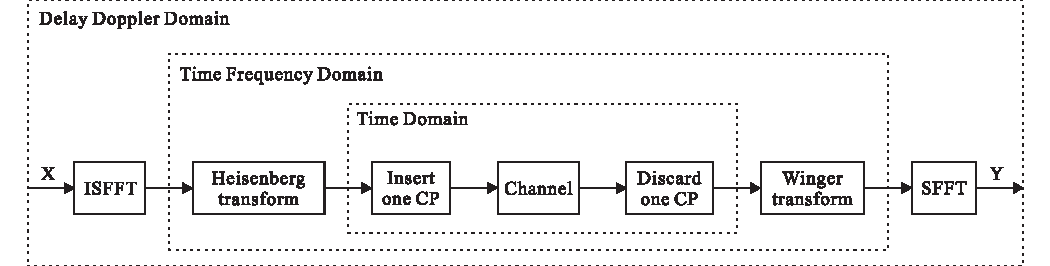
\includegraphics[width=\textwidth]{otfs_sys}
  \caption{OTFS mode/demod}
  \label{fig:otfs-sys}
\end{figure}
We consider a single input single output (SISO) OTFS system as illustrated in Fig.~\ref{fig:otfs-sys}. The transmitter operates an OTFS frame (detailed in \ref{sec:sys-frame}), $\mathbf X[k,l] \in \mathbb{C}^{K \times L}$, with $k = 0, \cdots, K-1$ and $l = 0, \cdots, L-1$ indexing discretized Doppler and delay shifts, respectively. After transposition. the frame is converted to the time-frequency (TF) domain via the inverse symplectic finite Fourier transform (ISFFT), mapping the data on $L\times K$ grids with uniform intervals $\Delta f$ (Hz) and $T=1/\Delta f$ (seconds).  The time-domain signal is synthesized using (discrete) Heisenberg transform with a pulse-shaping waveform employing a single initial cyclic prefix spanning the full OTFS frame duration. The time-domain signal is transmitted over a time-varying wireless channel characterized by the delay-Doppler impulse response $h(\tau, v)$ as \cite{7925924},
\begin{equation}
h(\tau, v) = \sum_{i=1}^P h_i \delta (\tau - {\tau}_i) \delta (v - v_i) ,
\end{equation}
where $\delta(\cdot)$ denotes the Dirac delta function, $h_i \sim \mathcal{N}(0, \frac{1}{P})$ is the gain of the $i$-th propagation path, and $P$ represents the total number of paths. Each path is characterized by distinct delay and/or Doppler shifts, modeling the channel response between the receiver and either moving reflectors or the transmitting source. The delay and Doppler shifts are given as,
\begin{equation}
{\tau}_i = l_i \frac{T}{L}, v_i = k_i \frac{\Delta f}{K},
\end{equation}
respectively. Let the integers $l_i \in [0, l_\max]$ and $k_i \in [-k_\max, k_\max]$ represent the delay and Doppler shift indices, respectively, where $l_\max$ and $k_\max$ denote the maximum delay index and maximum Doppler shift index across all propagation paths. Note that we restrict our consideration to integer-valued indices, as fractional delay and Doppler shifts can be equivalently represented through virtual integer taps in the delay-Doppler domain using the techniques described in \cite{6563167, 8377159, 8516353}.

\subsection{OTFS Frame Structure}\label{sec:sys-frame}
As illustrated in Fig.~\ref{fig:otfs-frame}, a superimposed OTFS frame structure is considered, where pilot and data symbols are jointly embedded over delay-Doppler grids, i.e.,
\begin{equation}
\mathbf{X} = \mathbf{X}_d + \mathbf{X}_p,
\end{equation}
where $\mathbf X_d[k, l] \in \mathbb{C}^{K \times L}$ denotes the data frame composed of quadrature amplitude modulation (QAM) symbols drawn from a constellation $\mathcal{A}$ with average energy $E_d$. The pilot frame $\mathbf X_p[k, l]$ contains nonzero elements only at designated positions, i.e.,
\begin{equation}
\mathbf X_p[k, l] =
\begin{cases}
x_p, & k = k_p,\ l = l_p, \\
0, & \text{otherwise},
\end{cases}
\end{equation}
where $x_p$ is the pilot symbol with energy $E_p$, $k_p = \lfloor (K-1)/2 \rfloor$ is the Doppler index of all pilots, and $l_p = i(l_\max + 1)$ for $i = 0, \dots, N_p - 1$ are their delay indices. Here, $N_p = \lfloor L / (l_\max + 1) \rfloor$ denotes the total number of pilots. Each pilot facilitates channel estimation over a region of size $K \times (l_\max + 1)$ in the DD domain.

\begin{figure}[H]
  \centering
  \includegraphics[scale=1]{otfs_frame}
  \caption{OTFS frame structure with the last pilot delay index at $l_{p,\text{last}} = (N_p - 1)(l_\max + 1)$}
  \label{fig:otfs-frame}
\end{figure}


\section{Variational Bayes in QJCHESD}
\subsection{OTFS Channel Estimation using VB}
We assume the channel follows the Gaussian distribution, i.e.,
\begin{equation}
p(h|\gamma) = \prod_{i=0}^{P_{\max}-1}p(h_i|\gamma_i) = \prod_{i=0}^{P_\max-1}\mathcal{CN}(h_i;0, \gamma_i^{-1}),
\end{equation}
where $P_\max=(l_\max+1)(2k_\max+1)$, $\gamma=[\gamma_0,\gamma_1,\cdots,\gamma_{P_\max-1}]$ is the precision vector of $h$. $\gamma$ follows the Gamma distribution, i.e.,
\begin{equation}
p(\gamma)=\text{Gamma}(\gamma; a, b)
\end{equation}
where $a$ is the shape parameter and $b$ is the inverse scale parameter. Also, we assume the noise obeys the Gaussian distribution, i.e.,
\begin{equation}
p(z)=\mathbf z \sim \mathcal{CN}(0, \alpha^{-1}\bm I)
\end{equation}
where $\alpha$ obeys the Gamma distribution, i.e.,
\begin{equation}
p(\alpha)=\text{Gamma}(\alpha; c, d)
\end{equation}
where $c$ is the shape parameter and $d$ is the inverse scale parameter. For all parameters, we define $\Theta=\{h,\gamma, \alpha\}$.

Here, we use the mean field assumption to estimate the channel, i.e.,
\begin{equation}
\begin{split}
p(y, \Theta) &= p(y|h,\alpha)p(h|\gamma)p(\gamma)p(\alpha) \\
lnp(y, \Theta) &= lnp(y|h,\alpha) + lnp(h|\gamma) + lnp(\gamma) + lnp(\alpha)
\end{split}
\end{equation}
Here, we use a distribution family $Q$ over $\Theta$ to approximate $p(\Theta|y)$, i.e.,
\begin{equation}
\begin{split}
p(\Theta|y) &= \mathop{\arg\min}\limits_{q(\Theta)\in Q} KL(q(\Theta) || p(\Theta|y)) \\
&= \mathop{\arg\min}\limits_{q(\Theta)\in Q} -\int_{\Theta}q(\Theta)\text{ln} \frac{p(\Theta|y)}{q(\Theta)}d\Theta
\end{split}
\end{equation}
where $q(\Theta)$ follows the mean field assumption, i.e.,
\begin{equation}
q(\Theta) = q(h)q(\gamma)q(\alpha)
\end{equation}
Therefore, we can update the probability functions as follows:
\begin{equation}
q^{(t+1)}(\alpha) \propto exp( \mathbb{E}_{q^{(t)}_{-\alpha}}[\text{ln}p(y,\Theta)] \} )
\end{equation}
\begin{equation}
q^{(t+1)}(h) \propto exp( \mathbb{E}_{q^{(t)}_{-h}}[\text{ln}p(y,\Theta)] \} )
\end{equation}
\begin{equation}
q^{(t+1)}(\gamma) \propto exp( \mathbb{E}_{q^{(t)}_{-\gamma}}[\text{ln}p(y,\Theta)] \} )
\end{equation}
The update is computed as follows
\begin{enumerate}[label=\arabic*)]
    \item Update $q(\alpha)$
    	\begin{align}
    	q^{(t+1)}(\alpha) &\propto exp( \mathbb{E}_{q^{(t)}_{-\alpha}}[\text{ln}p(y, \Theta)] \} ) \\
    	lnq^{(t+1)}(\alpha) &\propto \mathbb{E}_{q^{(t)}_{-\alpha}}[\text{ln}p(y, \Theta)] \\
    	lnq^{(t+1)}(\alpha) &\propto \mathbb{E}_{q^{(t)}_{h}}[\text{ln}p(y|h, \alpha)] + lnp(\alpha)
    	\end{align}
    	Here, 
    	\begin{align}
    	p(y|h, \alpha) &= \mathcal{CN}(\bm y_p; \bm\Phi_p\bm h, \alpha^{-1}\bm I) \notag \\
    	&= \frac{1}{\pi^Zdet(\alpha^{-1}\bm I)}e^{-(\bm y_p - \bm\Phi_p \bm h)^H(\alpha^{-1}\bm I)^{-1}(\bm y_p - \bm\Phi_p \bm h)} \\
    	&= \frac{1}{\pi^Zdet(\alpha^{-1}\bm I)}e^{-\alpha(\bm y_p - \bm\Phi_p \bm h)^H(\bm y_p - \bm\Phi_p \bm h)} \\
    	&= \frac{1}{\pi^Zdet(\alpha^{-1}\bm I)}e^{-\alpha \Vert \bm y_p - \bm\Phi_p \bm h\Vert^2}
    	\end{align}
    	where $Z$ is the dimension of $\bm y_p$.
    	Here, 
    	\begin{align}
    	det(\alpha^{-1}\bm I) = (\alpha^{-1})^Z = \alpha^{-Z}
    	\end{align}
    	Therefore,
    	\begin{align}
    	lnp(y|h, \alpha) &\propto Zln(\alpha) - \alpha \Vert \bm y_p - \bm\Phi_p \bm h\Vert^2 \\
    	\mathbb{E}_{q^{(t)}_{h}}\{lnp(y|h, \alpha)\} &\propto \mathbb{E}_{q^{(t)}_{h}}\{Zln(\alpha)\} - \mathbb{E}_{q^{(t)}_{h}}\{\alpha \Vert \bm y_p - \bm\Phi_p \bm h\Vert^2\}\\
    	\mathbb{E}_{q^{(t)}_{h}}\{lnp(y|h, \alpha)\} &\propto Zln(\alpha)  - \alpha\mathbb{E}_{q^{(t)}_{h}}\{\Vert \bm y_p - \bm\Phi_p \bm h\Vert^2\}
    	\end{align}
    	Now, we need to get $\mathbb{E}_{q^{(t)}_{h}}\{\Vert \bm y_p - \bm\Phi_p \bm h\Vert^2$,i.e.,
    	\begin{align}
    	\Vert \bm y_p - \bm\Phi_p \bm h\Vert^2 &= \bm y_p^H\bm y_p - \bm y_p^H\bm\Phi_p\bm h - \bm h^H\bm\Phi_p^H\bm y_p + \bm h^H\bm\Phi_p^H\bm\Phi_p\bm h \\
    	\mathbb{E}_{q^{(t)}_{h}}\{\Vert \bm y_p - \bm\Phi_p \bm h\Vert^2 &= \bm y_p^H\bm y_p - \bm y_p^H\bm\Phi_p\bm\mu_h - \bm\mu_h^H\bm\Phi_p^H\bm y_p + \mathbb{E}_{q^{(t)}_{h}}\{\bm h^H\bm\Phi_p^H\bm\Phi_p\bm h \}    	
    	\end{align}
    	Here, as in \cite{Wikipedia-QuadraticForm},
    	\begin{align}
    	\mathbb{E}_{q^{(t)}_{h}}\{\bm h^H\bm\Phi_p^H\bm\Phi_p\bm h \}   &= \bm\mu_p^H\bm\Phi_p^H\bm\Phi_p\bm\mu_p + \text{tr}(\bm\Phi_p^H\bm\Phi_p\bm\Sigma_h)\\
    	&= \bm\mu_p^H\bm\Phi_p^H\bm\Phi_p\bm\mu_p + \text{tr}\left( \bm\Phi_p\bm\Sigma_h\bm\Phi_p^H \right)
    	\end{align}
    	Therefore, 
    	\begin{align}
    	\mathbb{E}_{q^{(t)}_{h}}\{\Vert \bm y_p - \bm\Phi_p \bm h\Vert^2 &= \bm y_p^H\bm y_p - \bm y_p^H\bm\Phi_p\bm\mu_h - \bm\mu_h^H\bm\Phi_p^H\bm y_p + \bm\mu_p^H\bm\Phi_p^H\bm\Phi_p\bm\mu_p + \text{tr}(\bm\Phi_p^H\bm\Phi_p\bm\Sigma_h) \\
    	&= \Vert \bm y_p - \bm\Phi_p \bm\mu_h\Vert^2 + \text{tr}(\bm\Phi_p^H\bm\Phi_p\bm\Sigma_h)
    	\end{align}
    	Therefore, 
    	\begin{align}
    	lnq^{(t+1)}(\alpha) &\propto Zln(\alpha) - \alpha\left( \Vert \bm y_p - \bm\Phi_p \bm\mu_h\Vert^2 + \text{tr}(\bm\Phi_p^H\bm\Phi_p\bm\Sigma_h) \right)  + lnp(\alpha) \\
    	&\propto Zln(\alpha) - \alpha( \Vert \bm y_p - \bm\Phi_p \bm\mu_h\Vert^2 + \text{tr}(\bm\Phi_p^H\bm\Phi_p\bm\Sigma_h))  + (a-1)ln(\alpha) - b\alpha \\
    	&\propto (a + Z -1)ln(\alpha) - \alpha(b+ \Vert \bm y_p - \bm\Phi_p \bm\mu_h\Vert^2 + \text{tr}(\bm\Phi_p^H\bm\Phi_p\bm\Sigma_h)) 
    	\end{align}
    	Therefore,
    	\begin{align}
    	a^{(t+1)} &= a^{(t)} + z \\
    	b^{(t+1)} &= b^{(t)} + \Vert \bm y_p - \bm\Phi_p \bm\mu_h^{(t)})\Vert^2 + \text{tr}(\bm\Phi_p^H\bm\Phi_p\bm\Sigma_h^{(t)})
    	\end{align}
    	where $\Sigma_h^{(t)}$ and $\mu_h^{t}$ are the posterior covariance matrix and the posterior mean vector of $h^{(t)}$, which are both adjusted after updating $q(h)$.
    	The mean of $\alpha$ is
    	\begin{equation}
    	\hat{\alpha}^{(t+1)} = \frac{a^{(t+1)}}{b^{(t+1)}}
    	\end{equation}

    \item Update $q(h)$
	\begin{align}
	q^{(t+1)}(h) &\propto exp( \mathbb{E}_{q^{(t)}_{-h}}[\text{ln}p(y,\Theta)] \} ) \\
	lnq^{(t+1)}(h) &\propto \mathbb{E}_{q^{(t)}_{-h}}\{\text{ln}p(y,\Theta)\} \\
	&\propto \mathbb{E}_{q^{(t)}_{-h}}\{lnp(y|h,\alpha)\} + \mathbb{E}_{q^{(t)}_{-h}}\{lnp(h|\gamma^{(t)})\} \\
	&\propto -\mathbb{E}_{q^{(t)}_{-h}}\{\alpha\}\Vert \bm y_p-\bm\Phi_p\bm h \Vert^2 + \mathbb{E}_{q^{(t)}_{-h}}\{\bm\gamma^{(t)}\}\Vert \bm h \Vert^2 \\
	&\propto -\hat{\alpha}^{(t+1)} \Vert \bm y_p-\bm\Phi_p\bm h \Vert^2 -\bm h^H\text{diag}(\bm\gamma^{{-1}^{(t)}})^{-1}\bm h \\
	&\propto -\hat{\alpha}^{(t+1)} \Vert \bm y_p-\bm\Phi_p\bm h \Vert^2 - \bm h^H\text{diag}(\bm\gamma^{(t)})\bm h \\
	&\propto \hat{\alpha}^{(t+1)}\bm h^H\bm\Phi_p^H\bm y_p + \hat{\alpha}^{(t+1)}\bm y_p^H\bm\Phi_p\bm h - \hat{\alpha}^{(t+1)}\bm h^H\bm\Phi_h^H\bm\Phi_h\bm h - \bm h^H\text{diag}(\bm\gamma^{(t)})\bm h + \text{const} \\
	&\propto \hat{\alpha}^{(t+1)}\bm h^H\bm\Phi_p^H\bm y_p + \hat{\alpha}^{(t+1)}\bm y_p^H\bm\Phi_p\bm h - \bm h^H(\hat{\alpha}^{(t+1)}\bm\Phi_h^H\bm\Phi_h + \text{diag}(\bm\gamma^{(t)})\bm h + \text{const} \label{eq:qjchesd-che-qh-ln0}
	\end{align}    
	As in the assumption, $\bm h$ follows Guassian distribution, i.e.,
	\begin{align}
	q^{(t+1)}(\bm h) &= \mathcal{CN}\left( \bm h | \bm\mu_h^{(t+1)}, \bm\Sigma_h^{(t+1)} \right) \\ 
	lnq^{(t+1)}(\bm h) &\propto -(\bm h - \bm\mu_h^{(t+1)})^H\bm\Sigma_h^{(t+1)^{-1}}(\bm h - \bm\mu_h^{(t+1)}) \\
	&\propto \underbrace{\bm h^H\bm\Sigma_h^{(t+1)^{-1}}\bm\mu_h^{(t+1)} + \bm\mu_h^{(t+1)^H}\bm\Sigma_h^{(t+1)^{-1}}\bm h}_{linear} + \underbrace{\bm h^H\bm\Sigma_h^{(t+1)^{-1}}\bm h}_{quadratic} + \text{const}
	\end{align}
	Here, we can see that the covariance is 
	\begin{equation}
	\bm\Sigma_h^{(t+1)} = \left(\hat{\alpha}^{(t+1)}\bm\Phi_h^H\bm\Phi_h + \text{diag}(\bm\gamma^{(t)})\right)^{-1}
	\end{equation}
	Therefore, \eqref{eq:qjchesd-che-qh-ln0} can be written as
	\begin{align}
	lnq^{(t+1)}(h) &\propto \bm h^H \bm\Sigma_h^{(t+1)^{-1}} \left(\hat{\alpha}^{(t+1)}\bm\Sigma_h^{(t+1)} \bm\Phi_p^H\bm y_p\right) + \notag \\ 
	&\left(\hat{\alpha}^{(t+1)}\bm\Sigma_h^{(t+1)}\bm\Phi_p^H\bm y_p\right)^H\bm\Sigma_h^{(t+1)^{-1}}\bm h - \notag \\
	&\bm h^H\bm\Sigma_h^{(t+1)^{-1}}\bm h + \text{const}
	\end{align}
	Please note that the Hermitian matrix $\bm\Sigma_h^{(t+1)^H} = \bm\Sigma_h^{(t+1)}$. Therefore, the mean is 
	\[
	\bm\mu^{(t+1)} = \hat{\alpha}^{(t+1)}\bm\Sigma_h^{(t+1)} \bm\Phi_p^H\bm y_p
	\]
	
    
    \item Update $q(\gamma)$
    \begin{align}
    \text{ln}q^{(t+1)}(\gamma) &\propto \mathbb{E}_{q^{(t)}_{-\gamma}}\{\text{ln}p(y,\Theta)\} \\
    &\propto \mathbb{E}_{q^{(t)}_{-\gamma}}\{lnp(y|h,\alpha) + lnp(h|\gamma) + lnp(\gamma) + lnp(\alpha)\} \\
    &\propto \mathbb{E}_{q^{(t)}_{-\gamma}}\{lnp(h|\gamma) + lnp(\gamma)\} \\
    &\propto \sum_{l=0}^{P_\max-1} \left( ln(\gamma_l) - \gamma_l\Vert h_l^{(t+1)} \Vert^2 + (c-1)ln\gamma_l -d\gamma_l\right) \\
    &\propto \sum_{l=0}^{P_\max-1} \left( (\underbrace{c+1}_{c^{t+1}}-1)ln(\gamma_l) - \gamma_l \underbrace{(d + \Vert h_l^{(t+1)} \Vert^2)}_{d^{(t+1)}} \right)
    \end{align}
    where $\Vert h_l^{(t+1)} \Vert^2 = \Sigma_{h_l}^{t+1} + |\mu_{h_l}^{t+1}|^2$.
    Therefore,
    \begin{equation}
    \gamma = \text{diag}( \frac{c_0^{t+1}}{d_0^{(t+1)}}, \cdots,  \frac{c_{P_\max}^{t+1}}{d_{P_\max}^{(t+1)}})
    \end{equation}
    
    \item Initial values
    \begin{align}
    a^{(0)} &= b^{(0)} = 1 \\
    c^{(0)} &= d^{(0)} = 1
    \end{align}
 
\end{enumerate}
\subsubsection{Simplified OTFS Channel Estimation using VB}
If we assume the noise is known to us, the estimation process can be simplified as,
\begin{enumerate}[label=\arabic*)]
 \item Update $q(h)$
	\begin{align}
	q^{(t+1)}(h) &\propto exp( \mathbb{E}_{q^{(t)}_{-h}}[\text{ln}p(y,\Theta)] \} ) \\
	lnq^{(t+1)}(h) &\propto \mathbb{E}_{q^{(t)}_{-h}}\{\text{ln}p(y,\Theta)\} \\
	&\propto \mathbb{E}_{q^{(t)}_{-h}}\{lnp(y|h,\alpha)\} + \mathbb{E}_{q^{(t)}_{-h}}\{lnp(h|\gamma^{(t)})\} \\
	&\propto \alpha\bm h^H\bm\Phi_p^H\bm y_p + \alpha\bm y_p^H\bm\Phi_p\bm h - \bm h^H(\alpha\bm\Phi_h^H\bm\Phi_h + \text{diag}(\bm\gamma^{(t)})\bm h + \text{const}
	\end{align}    
	As in the assumption, $\bm h$ follows Guassian distribution, i.e.,
	\begin{align}
	q^{(t+1)}(\bm h) &= \mathcal{CN}\left( \bm h | \bm\mu_h^{(t+1)}, \bm\Sigma_h^{(t+1)} \right) \\ 
	lnq^{(t+1)}(\bm h) &\propto -(\bm h - \bm\mu_h^{(t+1)})^H\bm\Sigma_h^{(t+1)^{-1}}(\bm h - \bm\mu_h^{(t+1)}) \\
	&\propto \underbrace{\bm h^H\bm\Sigma_h^{(t+1)^{-1}}\bm\mu_h^{(t+1)} + \bm\mu_h^{(t+1)^H}\bm\Sigma_h^{(t+1)^{-1}}\bm h}_{linear} + \underbrace{\bm h^H\bm\Sigma_h^{(t+1)^{-1}}\bm h}_{quadratic} + \text{const}
	\end{align}
	Here, we can see that the covariance is 
	\begin{align}
	\bm\Sigma_h^{(t+1)} &= \left(\alpha\bm\Phi_h^H\bm\Phi_h + \text{diag}(\bm\gamma^{(t)})\right)^{-1} \\
	\bm\mu^{(t+1)} &= \alpha\bm\Sigma_h^{(t+1)} \bm\Phi_p^H\bm y_p
	\end{align}
	
	\item Update $q(\gamma)$
    \begin{align}
    \text{ln}q^{(t+1)}(\gamma) &\propto \mathbb{E}_{q^{(t)}_{-\gamma}}\{\text{ln}p(y,\Theta)\} \\
    &\propto \mathbb{E}_{q^{(t)}_{-\gamma}}\{lnp(y|h,\alpha) + lnp(h|\gamma) + lnp(\gamma) + lnp(\alpha)\} \\
    &\propto \mathbb{E}_{q^{(t)}_{-\gamma}}\{lnp(h|\gamma) + lnp(\gamma)\} \\
    &\propto \sum_{l=0}^{P_\max-1} \left( ln(\gamma_l) - \gamma_l\Vert h_l^{(t+1)} \Vert^2 + (c-1)ln\gamma_l -d\gamma_l\right) \\
    &\propto \sum_{l=0}^{P_\max-1} \left( \underbrace{(c+1-1)}_{c^{t+1}}ln(\gamma_l) - \gamma_l \underbrace{(d + \Vert h_l^{(t+1)} \Vert^2)}_{d^{(t+1)}} \right)
    \end{align}
    where $\Vert h_l^{(t+1)} \Vert^2 = \Sigma_{h_l}^{t+1} + |\mu_{h_l}^{t+1}|^2$.
    Therefore,
    \begin{equation}
    \gamma = \text{diag}( \frac{c_0^{t+1}}{d_0^{(t+1)}}, \cdots,  \frac{c_{P_\max}^{t+1}}{d_{P_\max}^{(t+1)}})
    \end{equation}	
	
\end{enumerate}


\subsection{Symbol Detection}
In this section, \colorbox{yellow}{we assume the channel is known}. The target is to find the channel and the symbol to maximize the posterior, i.e.,
\begin{equation}
\begin{split}
p(x; y, H, \sigma^2) &= \mathop{\arg\max}\limits_{x\in \Omega}  p(y|x; H, \sigma^2) p(x)
\end{split}
\end{equation}
Here, we use a 

\subsection{Joint Method}
We shall look at some examples to solve this problem

\begin{align}
||y_p-\phi_ph||^2 &= (y_p -\phi_ph)^H(y_p -\phi_ph) \\
&= y_p^Hy_p - y_p^H\phi_ph - (\phi_ph)^Hy_p  + (\phi_ph)^H(\phi_ph) \\
&= y_p^Hy_p - y_p^H\phi_ph - (\phi_ph)^Hy_p  + h^H\phi_p^H\phi_p h
\label{eq:jcesd-sbl-ce-alpha-0}
\end{align}
Here, 
\[
(y_p^H\phi_ph)^H = (\phi_ph)^Hy_p
\]
Therefore,
\[
y_p^H\phi_ph + (\phi_ph)^Hy_p = 2Re\{y_p^H \phi_p h\} 
\]
\[
||y_p-\phi_ph||^2 = y_p^Hy_p - 2Re\{y_p^H \phi_p h\}  + h^H\phi_p^H\phi_p h
\]
Now, we do the expectation for $||y_p-\phi_ph||^2$ on $h$,
\begin{align}
<||y_p-\phi_ph||^2>_h &= y_p^Hy_p - 2Re\{y_p^H \phi_p u_h\}  + <h^H\phi_p^H\phi_p h>_h\\
&= y_p^Hy_p - 2Re\{y_p^H \phi_p u_h\}  + <tr(h^H\phi_p^H\phi_p h)>_h \\
&= y_p^Hy_p - 2Re\{y_p^H \phi_p u_h\}  + <tr(\phi_p^H\phi_p hh^H)>_h \\
&= y_p^Hy_p - 2Re\{y_p^H \phi_p u_h\}  + tr(\phi_p^H\phi_p <hh^H>_h) \\
\end{align}
The covariance of $h$ is, 
\[
\Sigma_h = <hh^H> - u_h u_h^H
\]
\[
<hh^H> = \Sigma_h + u_h u_h^H
\]
Therefore,
\begin{align}
<||y_p-\phi_ph||^2>_h &= y_p^Hy_p - 2Re\{y_p^H \phi_p u_h\}  + tr(\phi_p^H\phi_p (\Sigma_h + u_h u_h^H)) \\
&= y_p^Hy_p - 2Re\{y_p^H \phi_p u_h\}  + tr(\phi_p^H\phi_p \Sigma_h) + tr(\phi_p^H\phi_p u_h u_h^H) \\
&= y_p^Hy_p - 2Re\{y_p^H \phi_p u_h\}  + tr(\phi_p^H\phi_p \Sigma_h) + tr(u_h^H\phi_p^H\phi_p u_h) \\
&= y_p^Hy_p - 2Re\{y_p^H \phi_p u_h\}  + u_h^H\phi_p^H\phi_p u_h + tr(\phi_p^H\phi_p \Sigma_h) \\
&= ||y_p - \phi_p u_h||^2 + tr(\phi_p \Sigma_h\phi_p^H)
\end{align}

\newpage
\bibliographystyle{IEEEtran}
\bibliography{./reference}
\end{document}